\section{Observations}\label{sec:observations}
This study encompasses a total of $44$ targeted pointings, where each pointing consists of a 15-minute scan centered on specific targets selected from the \textit{TESS} catalog, focusing on confirmed or candidate exoplanets (refer to Figure \ref{fig:TESS_TOIs}). The entire observation campaign spanned a duration of 11 hours, covering an area of 232 deg$^2$ in the northern sky. 

\begin{figure}[h!]
    \centering
    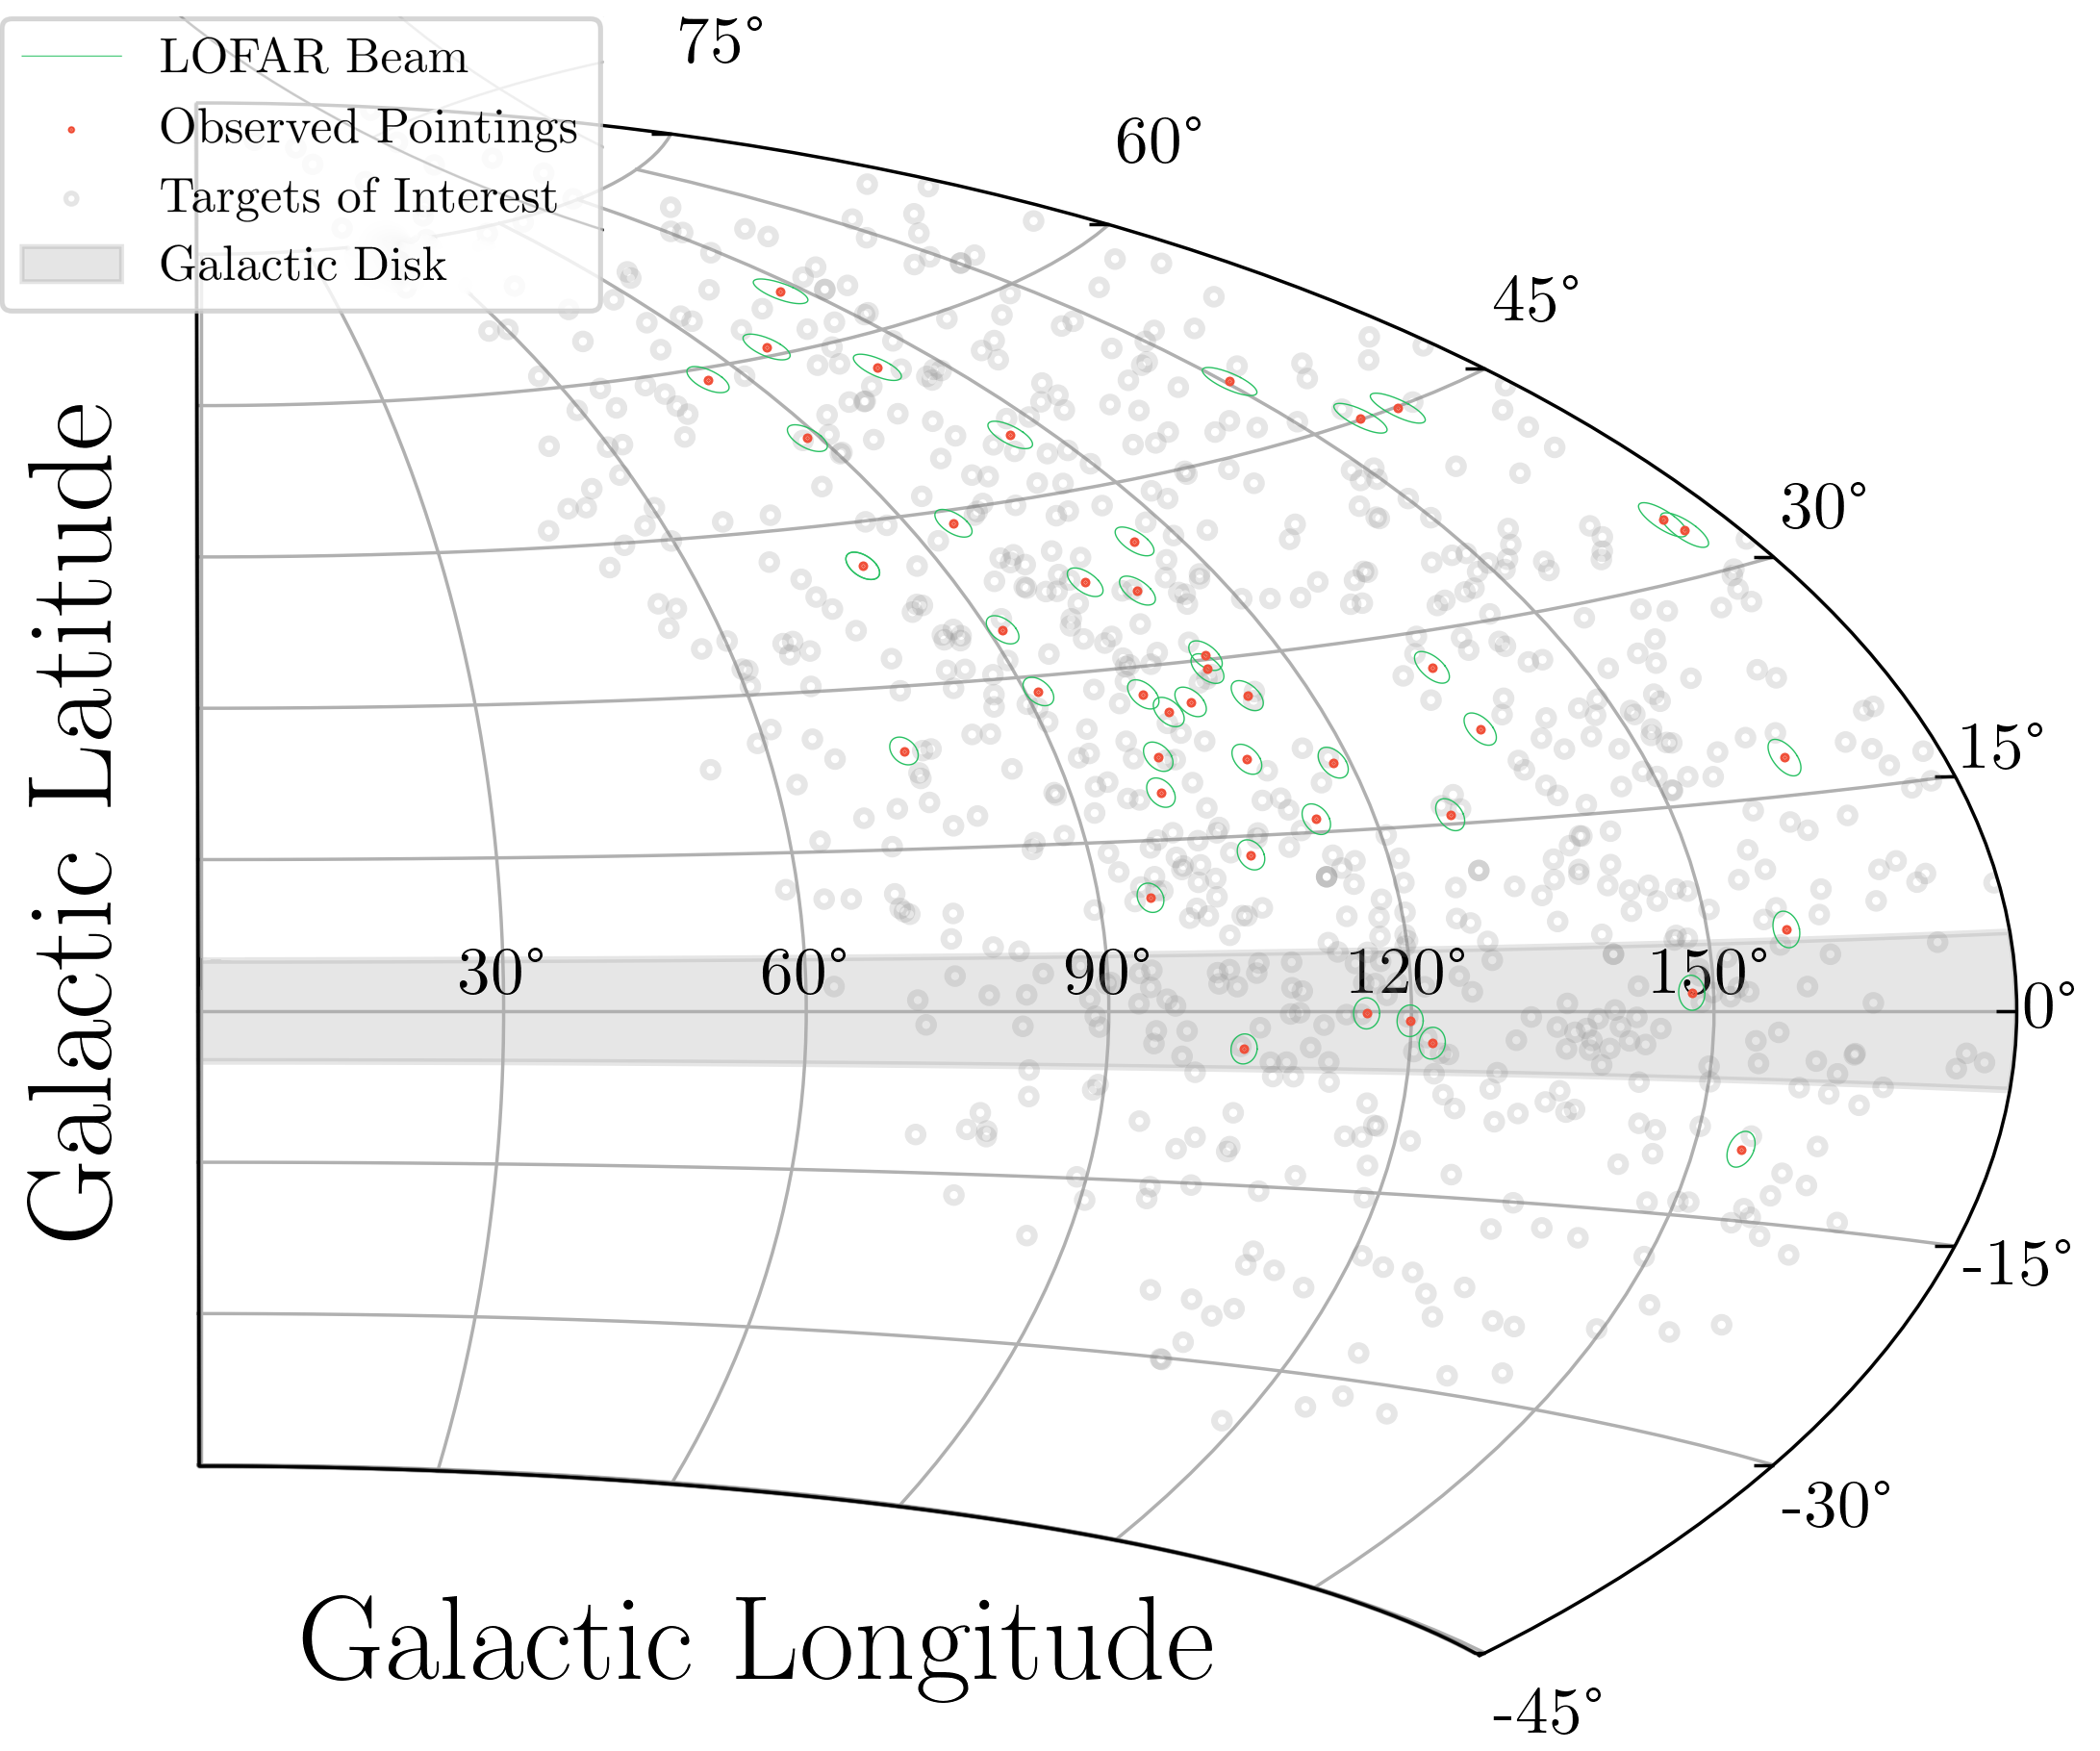
\includegraphics[width = 0.5\textwidth]{SETI/figures/TESS_progress/Aitoff_Projection_PSD.png}
    \caption{An Aitoff projection of the sky in Galactic coordinates depicts the distribution of survey pointings, with the Galactic disk shaded in grey. \textit{Gaia} sources are omitted from the plot due to their extremely high source density. Grey dots represent \textit{TESS} Targets of Interest (ToIs). Those targets observed during our survey are marked with red dots at boresight with green showing the half-power beam width ($2.59^\circ$).
  }
  \label{fig:TESS_TOIs}
\end{figure}

\subsection{LOFAR}
LOFAR, a pioneering low-frequency aperture array telescope, spans hundreds of kilometers across Europe and serves as a pathfinder to the Square Kilometer Array (SKA). The array consists of a core station with outrigger stations situated in the Netherlands and additional international stations spanning multiple countries, such as Germany, France, Sweden, Ireland, Latvia, Poland, and the United Kingdom. Additionally, stations are currently in the process of being constructed in Italy and Bulgaria. The LOFAR array operates using two types of antenna, the Low Band Antenna (LBA) and the High Band Antenna (HBA), operating at 10-90 MHz and 100-250 MHz respectively. In this study, the HBAs at the Irish and Swedish LOFAR station are used to carry out observations non-interferometrically.  The field-of-view (FoV) of an international LOFAR station is rather large; at full-width-half maximum it is $5.3$, $3.4$ and $2.3$ deg$^2$ at frequencies of $120$, $150$ and $180$~MHz, respectively~\citep{2013arXiv1305.3550V}. With such a large region where our observations are sensitive, each pointing contains millions of stars that can be searched for technosignatures \citep{Bart-Wlodarczyk-Sroka}. In this survey, in addition to the $44$ \textit{TESS} targets at boresight, \gaiatargets \textit{Gaia} targets are covered by our observations and so are searched for technosignatures. 

 \subsection{Targets} \label{sc:targets}

 A significant fraction of radio emission from Earth is emitted in the direction of the ecliptic plane. For example, powerful planetary radars are used to explore solar system objects \citep{Siemion_KEPLER_ApJ} and high-powered transmitters are used to communicate with solar system probes \citep{Enriquez:2017}. It is conceivable then that such leakage radiation may also be emanating from other worlds, preferentially in \textit{their} planetary orbital planes. This is why we chose \textit{TESS} targets, as these are the closest transiting exoplanet systems known \citep{kepler_2008,TESS_2015}. Observing these sources with the LOFAR HBAs enables robust constraints on any associated artificial low-frequency radio emission.  


\subsubsection{\textit{TESS} Targets} In order to determine a target list for this work, the latest list of \textit{TESS} object of interests (TOIs) was retrieved \citep{NEA12} and a shortlist of targets were obtained rejecting possible false positives. Since the sensitivity of the HBA array is best $\pm$30$^\circ$ of zenith, the required overlap for both LOFAR international stations spans the declination range +27$^\circ$ to +83$^\circ$. Further practical considerations were also accounted for, i.e. to stay as far from bright sources like the Sun as possible at both sites, and to balance sensitivity at both sites \citep{D-SOP}\footnote{These selection criteria were applied using a custom developed dual-site observation planning software.}. We report observations towards 44 unique targets from the \textit{TESS} catalogue in this study, where each target was observed for 15 minutes. Figure \ref{fig:TESS_TOIs} shows the distribution of these targets observed in comparison to the pool of all \textit{TESS} TOIs. 

\subsubsection{Gaia Sources}
The beam of a LOFAR station has an expansive coverage enabling observation of a substantial number of stars in the field-of-view. The significance of these in-field stars has been highlighted by \cite{Bart-Wlodarczyk-Sroka}. Consequently, during our observations targeting 44 sources from the TESS catalogue, we encountered a significant number of in-field stars within our field-of-view as shown in Figure \ref{fig:inbeam_trgts_SDSS}. 

\begin{figure}
    \centering
    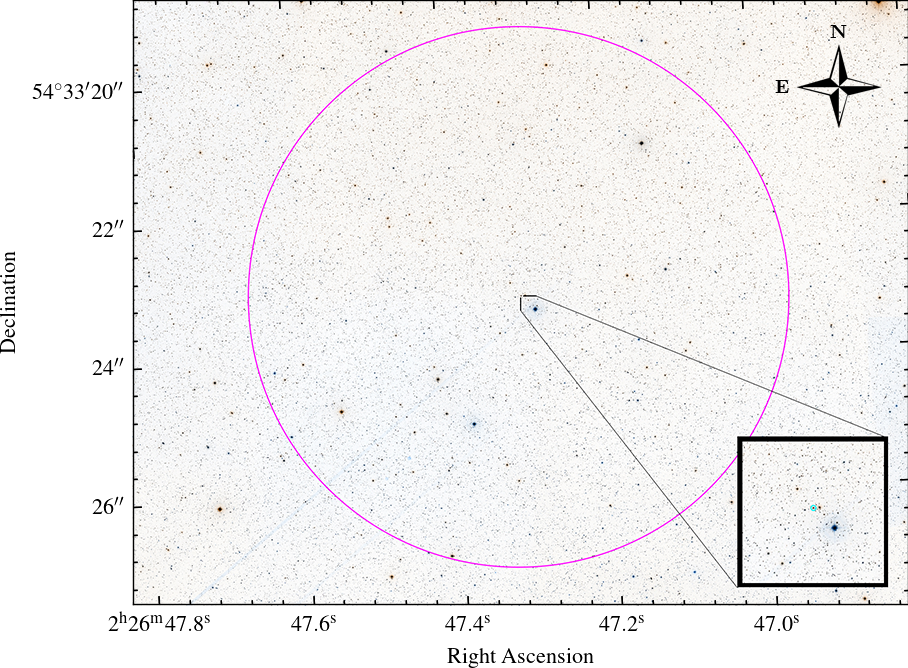
\includegraphics[width = 0.9\textwidth]{SETI/figures/EIRP_plots/frame.png}
    \caption{This figure illustrates one of the boresight pointings directed at a \textit{TESS} object (highlighted in green), with the LOFAR beam's Full-Width Half-Maximum (FWHM) shown in pink. The background image is from the Sloan Digital Sky Survey \citep[SDSS;]{SDSSDR13}.}
    \label{fig:inbeam_trgts_SDSS}
\end{figure}


To determine the list of targets within this field-of-view, we utilized the \textit{Gaia} catalogue. Some previous major SETI surveys focused their searches towards Sun-like stars \citep{Tarter:1996jf}. However, since our understanding of the origin of life is limited, it makes sense to allow for the possibility of life arising on a planet that is neither Earth-like, nor around stars that are Sun-like. Similarly, we should consider planets not necessarily located in the habitable zone. This is typically characterized as the orbital range wherein liquid water could exist~\citep{KASTING1993108}, as inferred from planetary equilibrium temperatures often ignoring the unknown albedo of the exoplanets. Any sensitive radio SETI survey seeking to maximize the chance of detecting weak radio signals should, insofar as possible, expand its search to encompass nearby stars of a broad range of spectral types and with exoplanets of all sizes and distances from their parent star. Thus, we conducted calculations to determine the number of \textit{Gaia} stars with a mean distance of 1215 pc, with an accuracy in their distances of at least 20\%. \\

This study used \textit{Gaia}'s third data release  \citep[GDR3;][]{2023GDR3, astroquery}. When analyzing GDR3 two filters were applied to the in beam target values survey volume and sensitivity accuracy. Firstly a constraint on the RA and DEC errors were implemented. If a \textit{Gaia} source was found to be in the beam but had a error magnitude greater than the FWHM it was removed from the source pool. \Cref{eq:condition1} states the first condition of filtering. 
% 7,818,294 -> 3,610,057 
\begin{equation}
    \theta_\text{sep} + \sqrt{\Delta \text{RA}^2 + \Delta \text{DEC}^2} < 1.295^\circ 
    \label{eq:condition1}
\end{equation}
As the sensitivity of the survey is calculated based on a source's distance a second filter is implemented to remove sources that have large errors. By taking the difference $(\Delta \sigma_G)$ in the upper and lower confidence levels of GSP-Photometry\footnote{SQL Keys: \texttt{distance\_gspphot}, \texttt{distance\_gspphot\_upper} $(d_{M_G})$ and \texttt{distance\_gspphot\_lower}} to obtain a percentage error on distance. All sources with a $d_{M_G}$ error of 20\% or greater are filtered out of the source list. Equation (\ref{eq:condition2}) states the second condition of filtering:
\begin{equation}
    \dfrac{\Delta \sigma_G}{d_{M_G}} < 20\% 
    \label{eq:condition2}
\end{equation}
A total of $\gaiatargets$ stars from this list, making it one of the largest samples of stars ever surveyed for SETI purposes. Figure~\ref{fig:HR-Diagram} shows a Hertzsprung-Russell diagram for the targets. 

\begin{figure}
    \centering
    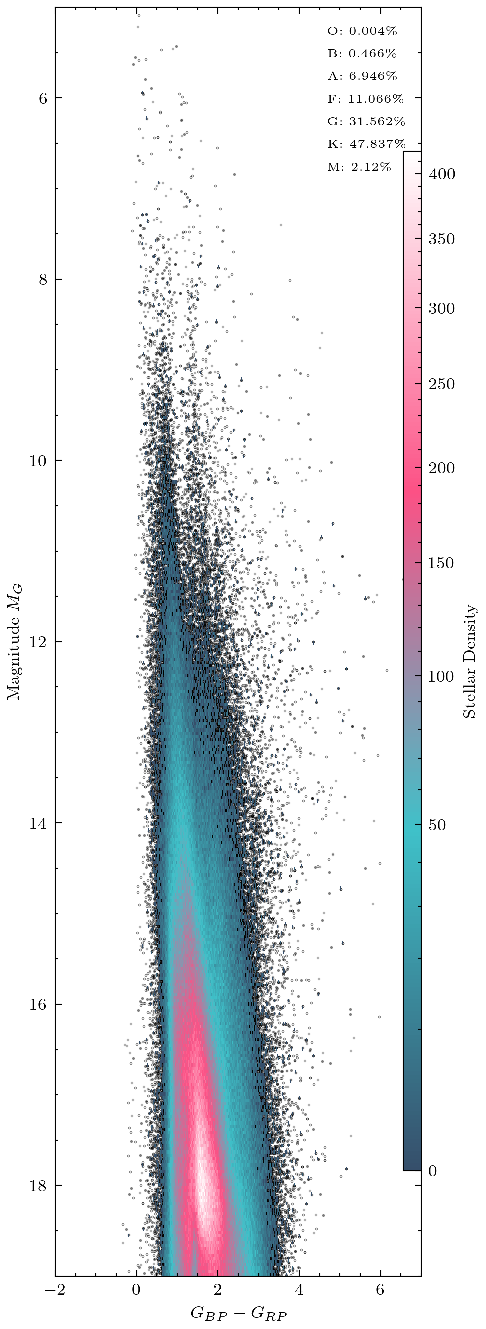
\includegraphics[width = 7cm]{SETI/figures/HR-diagram/HRD.pdf}
    \caption{A Hertzsprung-Russell diagram of the \surveytargets \textit{Gaia} targets searched for technosignatures in this survey with a mean distance of \distance pc. The relative distribution with respect to spectral type is: O $<0.01\%$, B---$0.4\%$, A---6.94\%, F---11.01\%, G---31.56\%, K---47.84\%, M---2.12\%. This is as opposed to the general \textit{Gaia} catalogue which is: O, B $<0.0001\%$, A---1.5\%, F---18.9\%, G---44.4\%, K---34.5\%, M---0.6\%.}
    \label{fig:HR-Diagram}
\end{figure}

\begin{figure}
    \centering
    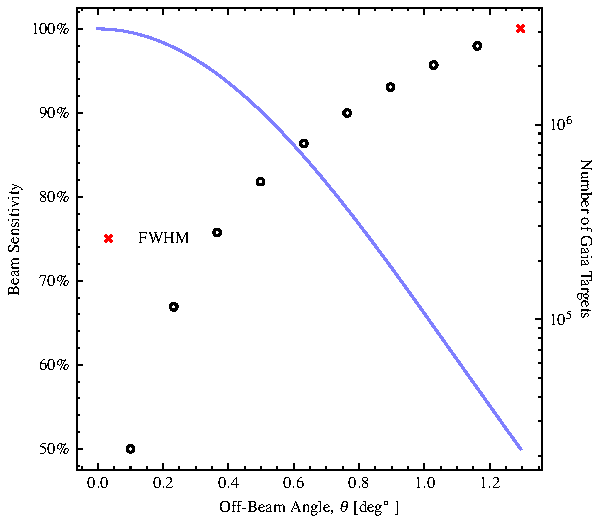
\includegraphics[width = 0.45\textwidth]{SETI/figures/EIRP_plots/off-beam-sensitivity-plots.pdf}
    \caption{The LOFAR HBA beam's sensitivity at 150~MHz changes in relation to the off-axis bore-sight angle ($\theta$). Furthermore, a plot of the number of filtered \textit{Gaia} targets within the beam pointing as a function of $\theta$ is presented. The \textcolor{red}{$\times$} represents the value for the Full Width Half Max of the beam.}
    \label{fig:off_beam_sens}
\end{figure}


\subsection{Simultaneous observations}

\begin{figure*}
    \centering
    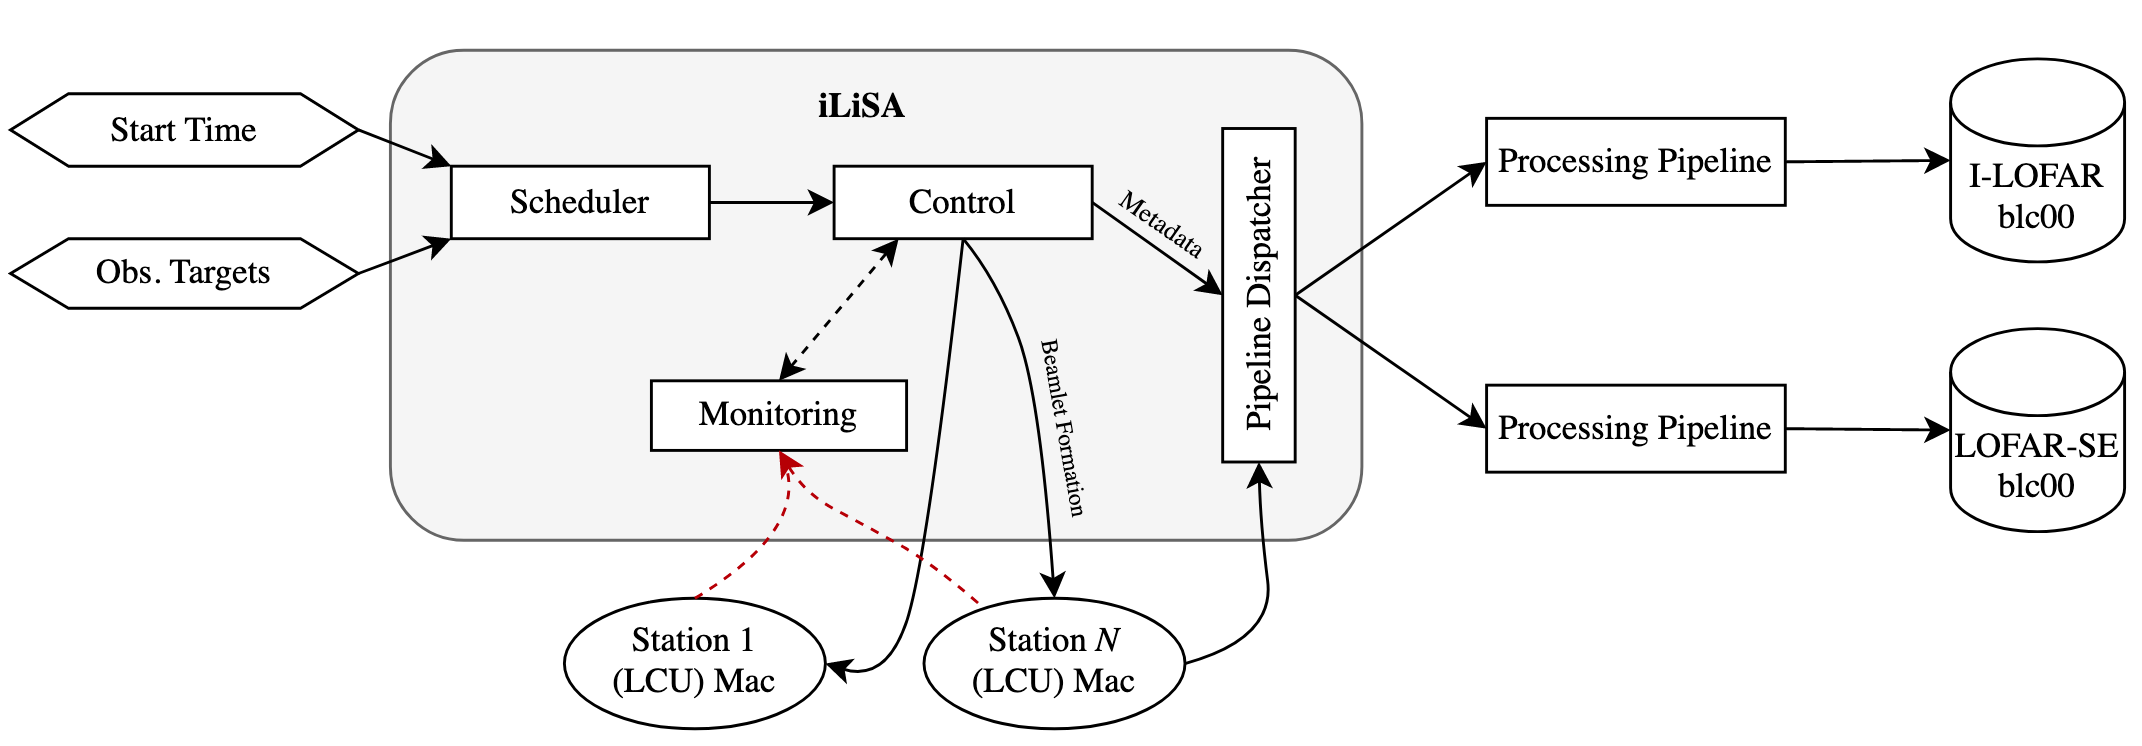
\includegraphics[width = 0.9\textwidth]{SETI/figures/iLiSA_Block_Diagramv2.png}
    \caption{\texttt{iLiSA} block diagram, showing how an operator-defined schedule is ingested and is executed in a timely fashion. Data then begins to flow and ends up being ingested by processing pipelines together with associated metadata.} %\textbf{Vishal to look over.}}
    \label{fig:iLiSA}
\end{figure*}

Typically, international LOFAR stations operate as standalone telescopes $2-3$ days per week, i.e. they do not operate as part of the International LOFAR Telescope's Europe-wide array. This project was undertaken during this standalone time. For this purpose the \emph{international LOFAR in Stand-Alone mode} (\texttt{iLiSA}) package\footnote{\url{https://github.com/2baOrNot2ba/iLiSA/releases/tag/v6.1}} is used to control both telescopes simultaneously. \texttt{iLiSA} provides a high-level operational control of multiple LOFAR stations, including scheduling, processing pipeline dispatching and metadata aggregation (see Figure~\ref{fig:iLiSA}). For the observations in this study, an operator-produced list of targets that were close\footnote{In practice as Birr and Onsala are separated by $\sim20\deg$ of longitude, the optimum scheduling is to observe $\sim 40$~min$-T_{\rm obs}/2$ `late' at Onsala and $40$~min$+T_{\rm obs}/2$ `early' at Birr.} to the local meridian was fed into \texttt{iLiSA} at each epoch. Towards each target, one beam per station was formed using \texttt{iLiSA}, and each beam was formed with $412$ HBA sub-bands (corresponding to a bandwidth of $80.46875$~MHz). The scan time on each target was $15$~min, and the whole scheduling block was a few hours per epoch.
% % for the record here is a filterbank header
% %Data file                        : TIC317597583.bary.0000.fil
% %Header size (bytes)              : 362
% %Data size (bytes)                : 144832462848
% %Data type                        : filterbank (barycentric)
% %Telescope                        : ???????
% %Datataking Machine               : ?????
% %Source Name                      : TICObj
% %Source RA (J2000)                : 23:28:04.0
% %Source DEC (J2000)               : +75:33:09.4
% %Frequency of channel 1 (MHz)     : 109.957138246395914
% %Channel bandwidth      (MHz)     : 0.000002980232239
% %Number of channels               : 27000832
% %Number of beams                  : 1
% %Beam number                      : -1
% %Time stamp of first sample (MJD) : 59402.347961288506
% %Gregorian date (YYYY/MM/DD)      : 2021/07/07
% %Sample time (us)                 : 671088.64000
% %Number of samples                : 1341
% %Observation length (minutes)     : 15.0
% %Number of bits per sample        : 32
% %Number of IFs                    : 1


%\subsection{The Data}
In this study, the only \texttt{iLiSA} pipeline used was the raw data recorder, which simply receives UDP packets of beam-formed data and writes them to disk, separately at each site. The data consist of coarse-channelised complex voltages. The initial data stream is two polarization's from each antenna. With real Nyquist-sampling with a $200$-MHz clock, with a coarse channelisation factor of $512$ taking place, only $488$ ($244$) of these being recordable when the data are written as 8-bit (16-bit) complex numbers. Further processing of these data is necessary and we use \texttt{udpPacketManager}~\citep{David_JOSS} to ultimately create total intensity  \texttt{sigproc} \citep{lorimerSIGPROCPulsarSignal2011} formatted filterbank files at the time and frequency resolution appropriate for our Doppler-drift search, shown in Table~\ref{tab:data_details}.

\begin{table}[ht]
\centering
\begin{tabular}{ll}
\hline
\textbf{Data Attribute} & \textbf{Value} \\
\hline
Frequency Start $(f_\text{start})$ & 109.9609375 MHz \\
Frequency End $(f_\text{end})$ & 190.0390625 MHz \\
Frequency Resolution & $2.980232239$~Hz \\
Channel Number & 27000832 \\
Obs. Length ($t_{\mathrm{obs}}$) & 15 mins \\
Temporal Resolution & $0.67108864$~s \\
Maximum Drift Rate Search & $\pm4 \ \text{Hz s}^{-1}$ \\
$\text{S}/\text{N}_{\text{min}}$ threshold & 10 \\
\hline
\end{tabular}
\caption{Specifications for the data input to our processing pipeline after pre-processing and preparing the raw data with \texttt{udpPacketManager}~\citep{David_JOSS}.}
\label{tab:data_details}
\end{table}

\begin{figure}
    \centering
    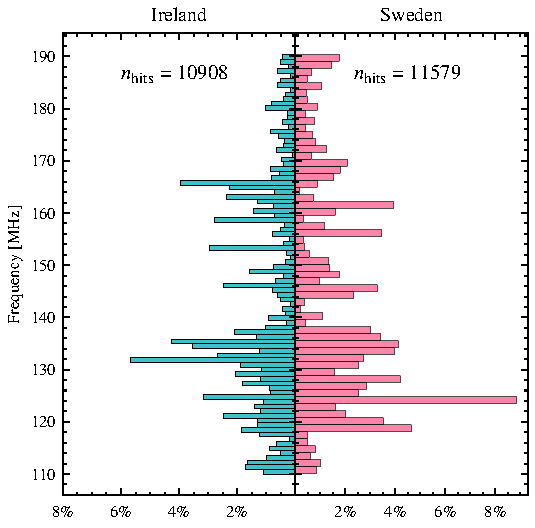
\includegraphics[width = 0.32\textwidth]{SETI/figures/narrowband/hits_comparative_histogram.pdf}
    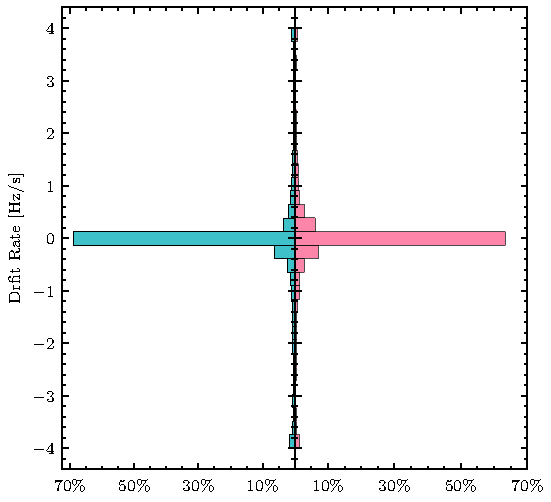
\includegraphics[width = 0.32\textwidth]{SETI/figures/narrowband/DR_comparative_histogram.pdf}
    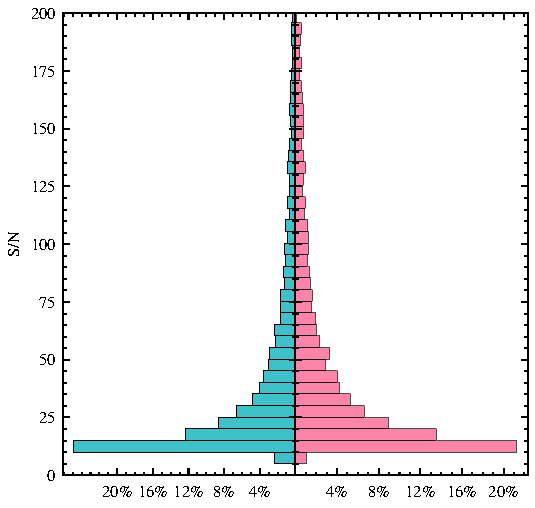
\includegraphics[width = 0.32\textwidth]{SETI/figures/narrowband/SN_comparative_histogram.pdf}
    \caption{Comparison of drifting signals or `hits' detected at both stations seen across the HBA frequency band. Each bin within the data set represents a 1 MHz frequency range and is accompanied by a corresponding percentage indicating its proportion to the overall data set.}
    \label{fig:histogram_hits_comparison}
\end{figure}
